% Created 2017-09-30 Sat 22:22
% Intended LaTeX compiler: pdflatex
\documentclass[presentation,9pt,xcolor=dvipsnames]{beamer}
\usepackage[utf8]{inputenc}
\usepackage[T1]{fontenc}
\usepackage{graphicx}
\usepackage{grffile}
\usepackage{longtable}
\usepackage{wrapfig}
\usepackage{rotating}
\usepackage[normalem]{ulem}
\usepackage{amsmath}
\usepackage{textcomp}
\usepackage{amssymb}
\usepackage{capt-of}
\usepackage{hyperref}
\institute{Post-doc (Georgetown University),PhD (Murdoch University)}
\usepackage{tikz}
\usepackage{color}
\usepackage{xcolor}
\usepackage{amsmath}
\usepackage{cancel}
\usepackage{graphicx}
\usetheme[height=7mm]{Rochester}
\usecolortheme[named=Green]{structure}
\usetikzlibrary{shapes,arrows}
\usetheme{default}
\author{Rob W Rankin}
\date{\today}
\title{Introduction to Bayesian Inference}
\hypersetup{
 pdfauthor={Rob W Rankin},
 pdftitle={Introduction to Bayesian Inference},
 pdfkeywords={},
 pdfsubject={},
 pdfcreator={Emacs 24.5.1 (Org mode 9.0.5)}, 
 pdflang={English}}
\begin{document}

\maketitle
\begin{frame}{Outline}
\tableofcontents
\end{frame}

\begin{frame}[label={sec:org51d5acb}]{themes}
see more themes in /usr/share/texlive/texmf-dist/tex/latex/beamer/themes/theme
\end{frame}
\begin{frame}[label={sec:org9ae5bef}]{outline}
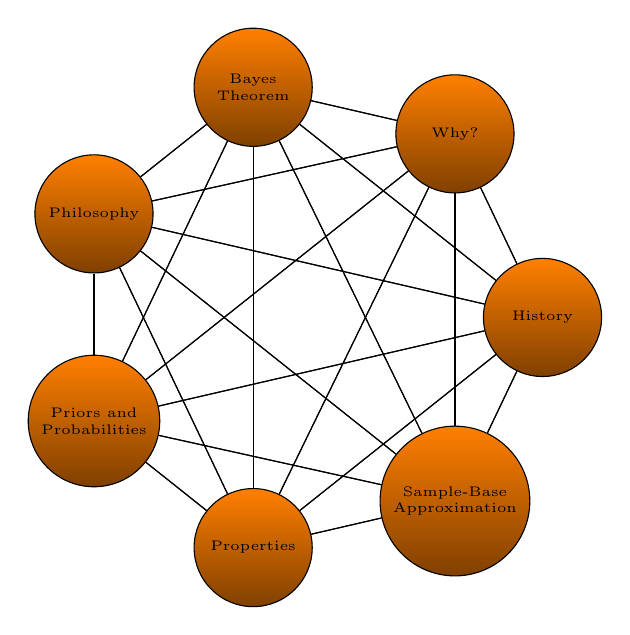
\begin{tikzpicture}
  \foreach \x /\alph/\name in {0/a/History, 51/b/Why?, 103/c/Bayes\\Theorem, 154/d/Philosophy, 206/e/Priors and\\Probabilities, 257/f/Properties, 309/g/Sample-Base\\Approximation}{
    \node[circle, fill=green,minimum width=15mm, draw, font=\tiny, align=center,shading=axis,top color=orange,bottom color =orange!50!black] (\alph) at (\x:3cm) {\name}; }

  \foreach \alpha in {a,b,c,d,e,f,g}%
           {%
             \foreach \alphb in {a,b,c,d,e,f,g}
                      {
                        \draw (\alpha) -- (\alphb);%
                      }
           }
\end{tikzpicture}
\end{frame}
\begin{frame}[label={sec:org2b21b51}]{Why?}
Why are you interested in Bayesianism?
\end{frame}
\begin{frame}[label={sec:org09cfbcc}]{Why? -- some advantages}
\begin{columns}
\begin{column}{0.55\columnwidth}
\begin{block}{Things Ecologist say\ldots{}}
\begin{itemize}
\item small sample sizes: exact inference
\item missing data: easy to impute
\item integrate other information
\item derived quantities
\item complex, hierarchical process models
\end{itemize}
multiple sources of variation (space,time)
``honest" epistemology
\end{block}
\end{column}
\begin{column}{0.45\columnwidth}
\begin{block}{Theoretical}
\begin{itemize}
\item conditional on the observed data
\item probabilistic statements
\item evidential
\item coherence, decision making
\item good frequentist properties
\end{itemize}
-- shrinkage, decision-theory
\begin{itemize}
\item model selection
\end{itemize}
\end{block}
\end{column}
\end{columns}
\end{frame}
\begin{frame}[label={sec:org2490bdd}]{Why? -- disadvantages}
\begin{itemize}
\item what is probability (basing inference on something that doesn't exist!!!)?
\item objective basis for science?
\item misalignment: probability theory and human psychology
\item bias (to prior)\footnote{Bayesian would claim that, if a prior exists, it would be irrational to believe in anything other than the posterior.}
\item language dependence
\end{itemize}
\end{frame}
\begin{frame}[label={sec:orgc90e9e1}]{History}
\begin{block}{Neo Bayesian Revival (>1992)}
Gelfand and Smith 1992 - Sampled based approximations of Bayesian posteriors \footnote{MCMC is older, e.g. Metrpolis et al. }
\end{block}
\begin{block}{Revival (\textasciitilde{}1920s - )}
Subjective Bayesian, Decision Theory
\begin{itemize}
\item Ramsey (1926)
\item De Finetti (1937)
\item Savage (1954)
\item (Wald, 1939, 1954)
\end{itemize}
Hypothesis Testing, Logical/Objective Bayesism
\begin{itemize}
\item Jeffreys (1939)
\item Jaynes (2003)
\end{itemize}
Hierarchical Bayesian
\begin{itemize}
\item Good (1953,65)
\end{itemize}
Relationship to Compact Coding Theory
\begin{itemize}
\item Rissasen (1978), Wallace (1968)
\end{itemize}
Prediction
\begin{itemize}
\item Dawid, Watanabe
\end{itemize}
\end{block}
\end{frame}
\begin{frame}[label={sec:org2828cc3}]{History - Frequentism's Ascendency}
\begin{block}{Frequentist ``lethal blow"\footnote{S. Zabell 1989}}
Rallied against use of prior probabilities in statistical inference
\begin{itemize}
\item Ronald A. Fisher (1925,1935,\ldots{})
\end{itemize}
Maximum likelihood, significance tesing, ANOVA, sufficiency, randomized experiments
\begin{itemize}
\item Jerzy Neyman \& Egon Pearson (1933)
\end{itemize}
Hypothesis testing, confidence intervals
\end{block}
\begin{block}{Falsificationism}
\begin{itemize}
\item Karl Popper (1959,1963)
\end{itemize}
\end{block}
\end{frame}
\begin{frame}[label={sec:org08bbeb7}]{History - Hypotheses}
\begin{columns}
\begin{column}{0.55\columnwidth}
\begin{block}{\uline{Frequentism}}
\begin{block}{Fisher's p-value}
\begin{itemize}
\item continuous index of evidence \alert{against} a hypothesis \(H\)
\item \alert{NEVER} prove a hypothesis \(H\), only disprove
\end{itemize}
\end{block}
\begin{block}{Neyman-Pearson \(\alpha\) and \(\beta\)}
\begin{itemize}
\item long-run error rates of Type-I and Type-II
\item \alert{bound} Type-I at \(\alpha\leq0.05\) and hopefully maximize power (\(1-\beta\)) with high \(n\) and most powerful tests
\item never confirm a hypothesis: only \alert{act} so as to ``not be wrong too often"
\end{itemize}
\end{block}
\end{block}
\end{column}
\begin{column}{0.45\columnwidth}
\begin{block}{\uline{Bayesians}}
\begin{block}{Model probabilities}
probabilistic confirmation of hypotheses
\begin{itemize}
\item \$p(H\(_{\text{k}} \vert Y)\) what is the probability of Hypothesis \(H_k\) given the data?
\end{itemize}
\end{block}
\begin{block}{Bayes Factors}
evidence in favour of one hypothesis over another
\begin{itemize}
\item \(BF=\frac{p(Y\vert H_1)}{p(Y\vert H_2)}\).
\end{itemize}
find hypothesis that is more likely to be true
\end{block}
\end{block}
\end{column}
\end{columns}
\end{frame}
\begin{frame}[label={sec:org4692681}]{History - Inverse Probability}
from late 1700's to \textasciitilde{}1920's: \uline{Method of Inverse Probability},the bread and butter of applied analyses
\begin{itemize}
\item Thomas Bayes (1778)
\item Laplace (1774)
\end{itemize}
\begin{block}{Bayes Theorem}
conditional probability
\begin{equation}
\overbrace{p(\theta\vert Y)}^{\text{posterior}} = \frac{\overbrace{p(\theta)}^{\text{prior}}\overbrace{\mathcal{L}(Y\vert \theta)}^{\text{likelihood}}}{\underbrace{f(Y)}_{\text{marginal likelihood}}} 
\end{equation}
\begin{itemize}
\item \textbf{Prior}: distribution of \(\theta\) (before the data)
\item \textbf{Likelihood}: joint probability density of the data (given \(\theta\))
\item \textbf{Posterior}: distribution of \(\theta\) (given the \(\theta\))
\item \(f(Y)\equiv \text{marginal likelihood}\ \int f(Y\vert\theta)p(\theta) d \theta\)
\end{itemize}
\end{block}
\end{frame}

\begin{frame}[label={sec:org2151a08}]{Bayes Theorem}
\ldots{}or more commonly,
\begin{equation}
\begin{aligned}
p(\theta\vert Y) & \propto f(Y\vert \theta)p(\theta) \\
\text{where} & \dots \\
& p(\theta)\equiv\text{prior information (before the data)} \\
& f(Y\vert\theta)\equiv\ \text{likelihood (information from the data)} \\
& p(\theta\vert Y) \equiv\text{distibuion of}\ \theta\ \text{after the  data} \\
& \cancel{f(Y)}\ \cancel{\text{marginal likelihood}}\text{(often ignore)}
\end{aligned}
\end{equation}
\begin{itemize}
\item posterior is a mixture of information in \alert{prior} and \alert{likelihood}
\end{itemize}
\end{frame}
\begin{frame}[label={sec:orgfd5d413}]{Bayesian Conditionalization}
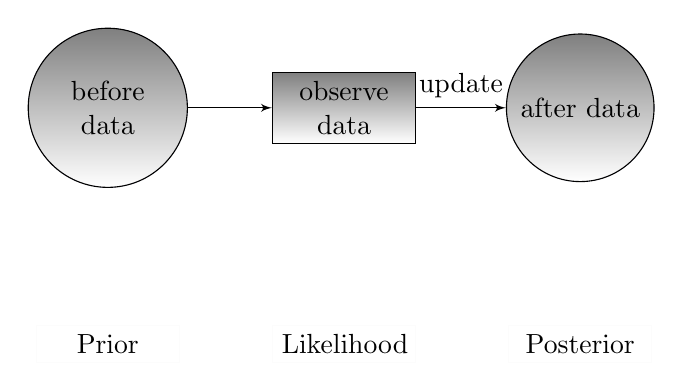
\begin{tikzpicture}[node distance = 3cm, auto]
  \node at (0,0) [rectangle, fill=blue, draw, text width=4.5em, align=center,shading=axis](likelihood){observe data};
  \node[circle, fill=blue, draw, text width=4.5em, align=center,shading=axis, left of = likelihood](prior){before data};
  \node[circle, fill=blue, draw, text width=4.5em, align=center,shading=axis, right of = likelihood](posterior){after data};
  \path [draw, -latex'] (prior) -- (likelihood); %
  \path [draw, -latex'] (likelihood) -- node{update} (posterior);
  \node[rectangle, draw, text width=4.5em, align=center,below of=likelihood,opacity=0.01,text opacity=1](likelabel){Likelihood};
  \node[rectangle, draw, text width=4.5em, align=center,below of=prior,opacity=0.01,text opacity=1](priorlabel){Prior};
  \node[rectangle, draw, text width=4.5em, align=center,below of=posterior,opacity=0.01,text opacity=1](postlabel){Posterior};    
\end{tikzpicture}
\end{frame}
\begin{frame}[label={sec:org5b06676}]{What's in a Posterior}
\begin{block}{Mixture of information}
\begin{itemize}
\item \(\mathcal{L}(Y\vert\theta)\): Likelihood, specified by model. Similar between Bayesian and non-Bayesian analyses\footnote{Frequentists reserve the term likelihood for a function of $\theta$ for fixed y, whereas Bayesians consider ``joint probability density of the data" given $\theta$.}
\item \(p(\theta)\) \ldots{} where do they come from?
\end{itemize}
\end{block}
\begin{block}{How to specify priors (HUGE topic)}
\begin{itemize}
\item a previous posterior distribution
\item elicitation from experts, previous studies
\item Priors as degrees-of-beliefs: \textbf{Subjectivist/personalist} Bayesians\}
\item Default prior and reference priors: \textbf{Objective/logical Bayesians}
\item adhoc
\end{itemize}
\end{block}
\end{frame}
\begin{frame}[label={sec:orga8393e9}]{Posterior Inference (for estimation \(\theta\))}
\begin{itemize}
\item Probabilistic statements about abstract quantity (\(\theta\)) (\emph{only} Bayesians can do)
\item Posterior probability necesarily depends on a \emph{prior}
\end{itemize}
``to make an Omelette, you must crack a few eggs" (Savage)
\begin{block}{The joy of Posterior Inference}
can make statements like\ldots{}
\begin{itemize}
\item what is the probability that \(\theta>0\)?
\item what is the most probable value of \(\theta\)? (\textcolor{red}{MAP})
\item what is the expected value of \(\theta\)? (\textcolor{red}{posterior mean})
\item what is a \emph{high probability region} of \(\theta\) (\textcolor{red}{Q\% credibility interval})
\end{itemize}
\end{block}
\end{frame}
\begin{frame}[fragile,label={sec:org4f3c69e}]{Posterior Inference (estimation example)}
 \begin{block}{Example 1:}
\begin{itemize}
\item men's height, n=20 observations.
\item \(y_i\sim\mathcal{N}(175,10^2)\)
\end{itemize}
\texttt{y <- c(183.46, 182.32, 178.31, 181.36, 165.12, 185.68, 170.47, 178.11, 174.86, 182.03, 180.09, 172.88, 177.94, 177.26, 182.58, 171, 173.74, 177.78, 180.02, 163.05)}
\begin{itemize}
\item estimate \(\theta=[\mu,\sigma^2]\): mean population height and variance
\item priors:  \(p(\mu)=\mathcal{N}(0,90^2),\ p(\sigma^2)=\mathcal{IG}(0.1,0.1)\)
\item specify a likelihood: \(\mathcal{L}(\mathbf{y}\vert\mu,\sigma^2)=\prod_i^n\mathcal{N}(y_i; \mu,\sigma^2)\)
\end{itemize}
\end{block}
\begin{block}{\emph{now run a Gibbs sampler to approximate the posterior} \(p(\mu,\sigma^2\vert \mathbf{y})\dots\)}
\end{block}
\end{frame}
\begin{frame}[label={sec:org45839ab}]{Posterior density}
\begin{itemize}
\item IS a probability distribution
\end{itemize}
\begin{center}
\includegraphics[width=0.6\textwidth,height=0.6\textheight]{posterior1.eps}
\end{center}
\begin{itemize}
\item easy to interpret
\end{itemize}
\end{frame}
\begin{frame}[label={sec:org4590f07}]{Posterior density}
\begin{itemize}
\item IS a probability distribution
\end{itemize}
\begin{center}
\includegraphics[width=0.6\textwidth,height=0.6\textheight]{posterior2.eps}
\end{center}
\begin{itemize}
\item Posterior mode: most probable value
\item Posterior mean \(\mathbb{E}[\theta]=\int p(\theta\vert Y)\theta d\theta\): expected value
\end{itemize}
\end{frame}
\begin{frame}[label={sec:org8190f0d}]{Posterior density}
\begin{itemize}
\item IS a probability distribution
\end{itemize}
\begin{center}
\includegraphics[width=0.6\textwidth,height=0.6\textheight]{posterior3.eps}
\end{center}
\begin{itemize}
\item Posterior mode: most probable value
\item Posterior mean \(\mathbb{E}[\theta]=\int p(\theta\vert Y)\theta d\theta\): expected value
\item 95\%CI of \(\theta\)
\end{itemize}
\end{frame}
\begin{frame}[label={sec:orga0441df}]{Posterior density}
\begin{itemize}
\item IS a probability distribution
\end{itemize}
\begin{center}
\includegraphics[width=0.6\textwidth,height=0.6\textheight]{posterior4.eps}
\end{center}
\begin{itemize}
\item Posterior mode: most probable value
\item Posterior mean \(\mathbb{E}[\theta]=\int p(\theta\vert Y)\theta d\theta\): expected value
\item What is the probability that \(\theta>X\)? Area of \(p(\theta\vert Y)>X\)
\end{itemize}
\end{frame}
\begin{frame}[label={sec:org9f6225b}]{Posterior Estimation vs Maximum Likelihood Estimation}
Bayesian vs. frequentist estimates: compare posteriors to maximum-likelihood method
\begin{block}{method of maximum likelihood}
\begin{itemize}
\item Choose \(\theta\) such that we \emph{maximize} the likelihood (\(\mathcal{L}\)) of seeing \(\mathbf{y}\)
\item \alert{interpretation} "It would be very (un)likely to see the data that I saw, if the value of \(\theta\) were X"
\item Most common method among Frequentists (single model estimation)
\item \(\hat{\theta}_\text{MLE}\) is \textcolor{red}{NOT} the "most probabilty value of \(\theta\)
\item \alert{optimality}: unbaised, efficient \footnote{but see shrinkage estimators for high-dimensional problems}
\end{itemize}
\end{block}
\end{frame}
\begin{frame}[fragile,label={sec:org661d2a3}]{Posterior Estimation vs Maximum Likelihood Estimation}
 \begin{center}
\includegraphics[width=0.6\textwidth,height=0.6\textheight]{loglike.eps}
\end{center}
\begin{itemize}
\item frequentist point estimates: \texttt{glm(y\textasciitilde{}1)}
\end{itemize}
\small
\begin{center}
\begin{tabular}{rrrr}
MLE & se & 95CI-low & 95CI-hi\\
172.3 & 1.48 & 169.4 & 175.17\\
\end{tabular}
\end{center}
\begin{itemize}
\item compare to (approximate)\footnote{some error due to Monte-Carlo approximation of the posterior.} Posterior descriptive statistics
\end{itemize}
\small
\begin{center}
\begin{tabular}{rrrr}
E[\(\theta\)] & SD & 95CI-low & 95CI-hi\\
172.21 & 1.51 & 169.21 & 175.16\\
\end{tabular}
\end{center}
nearly the same
\end{frame}
\begin{frame}[fragile,label={sec:org14aeedc}]{Posterior Inference (estimation example 2)}
 \begin{block}{Example 2:}
\begin{itemize}
\item survival \([0=\text{died},1=\text{survived}]\), \(n=30\) observations.
\item \(s_i\sim\text{Bern}(0.9)\)
\end{itemize}
\texttt{s <- c(1,1,1,1,0,1,0,1,1,1,1,1,1,1,1,0,1,0,1,1,1,1,1,1,1,1,1,1,1,1)}
\begin{itemize}
\item estimate \(\theta=[\phi]\): mean population survival
\item priors:  \(p(\phi)=\text{Beta}(1,1)\)
\item specify a likelihood: \(\mathcal{L}(\mathbf{s}\vert\phi,n_s)=\prod_s^n\text{Bern}(s_i; \phi,n_s)\)
\end{itemize}
\alert{now run a Gibbs sampler to approximate the posterior} \(p(\phi\vert \mathbf{s})\)
\end{block}
\end{frame}
\begin{frame}[label={sec:org56cfbcc}]{Posterior density}
\begin{center}
\includegraphics[width=0.6\textwidth,height=0.6\textheight]{posterior_s3.eps}
\end{center}
\end{frame}
\begin{frame}[label={sec:org96fb61b}]{Posterior density}
\begin{center}
\includegraphics[width=0.6\textwidth,height=0.6\textheight]{posterior_s4.eps}
\end{center}
\end{frame}
\begin{frame}[label={sec:orgf07d9c8}]{Posterior inference: cost functions}
What if you have a ``cost function" \(g(phi)\)?
e.g., cost of conservation action conditional on the estimated values of \(\phi\)?
\begin{center}
\includegraphics[width=0.7\textwidth,height=0.7\textheight]{surv_cost_func.eps}
\end{center}
\end{frame}
\begin{frame}[label={sec:org033ef5e}]{Posterior inference: cost functions}
\begin{center}
\includegraphics[width=0.7\textwidth,height=0.7\textheight]{surv_cost_est.eps}
\end{center}
\(\mathbb{E}[\text{COST}] = \int_0^1g(\phi)p(\phi\vert s)d\phi\)
\begin{itemize}
\item full cost including all uncertainty in \(\phi\)
\end{itemize}
\end{frame}
\begin{frame}[label={sec:org1a797d7}]{Posterior Estimation vs Maximum Likelihood Estimation}
How do Bayesian posterior estimates compared to more-familiar (frequentist) point-estimates based on maximum likelihood?
\begin{block}{method of maximum likelihood}
\begin{itemize}
\item Most common method among Frequentists (single model estimation)
\item "It would be very (un)likely to have seen the data that I saw, if the value of \(\theta\) were X"
\item Choose \(\theta\): that which \emph{maximize's} the likelihood of seeing \(\mathbf{y}\)
\item \(\hat{\theta}_\text{MLE}\) is \textcolor{red}{NOT} the "most probabilty value of \(\theta\)
\item optimality properties: unbaised, efficient \footnote{but see shrinkage estimators for high-dimensional problems}
\end{itemize}
\end{block}
\end{frame}
\begin{frame}[fragile,label={sec:org080b27d}]{Posterior Estimation vs Maximum Likelihood Estimation}
 \begin{center}
\includegraphics[width=0.6\textwidth,height=0.6\textheight]{loglike.eps}
\end{center}
\begin{itemize}
\item frequentist point estimates: \texttt{glm(y\textasciitilde{}1)}
\end{itemize}
\small
\begin{center}
\begin{tabular}{rrrr}
MLE & se & 95CI-low & 95CI-hi\\
172.3 & 1.48 & 169.4 & 175.17\\
\end{tabular}
\end{center}
\begin{itemize}
\item compare to (approximate)\footnote{some error due to Monte-Carlo approximation of the posterior.} Posterior descriptive statistics
\end{itemize}
\small
\begin{center}
\begin{tabular}{rrrr}
E[\(\theta\)] & SD & 95CI-low & 95CI-hi\\
172.21 & 1.51 & 169.21 & 175.16\\
\end{tabular}
\end{center}
nearly the same
\end{frame}

\begin{frame}[label={sec:org906d453}]{Posterior Estimation vs Maximum Likelihood Estimation}
\begin{block}{for \(n\) getting \alert{LARGE}, and for \alert{WEAK} priors}
\begin{itemize}
\item Posterior Mode \(\theta_{\text{MAP}}\rightarrow\hat{\theta}_{\text{MLE}}\)
\item Posterior Confidence Intervals \(\rightarrow\) Confidence Intervals
\end{itemize}
\end{block}
\begin{block}{for \alert{low} \(n\) and/or for \alert{STRONG} priors}
\begin{itemize}
\item shrinkage:  \(\theta\rightarrow\text{Prior expectation}\).
\item Posterior mean \(\bar{\theta}\) is ``biased" towards the priors
\end{itemize}
\end{block}
\begin{block}{role of priors (from an estimation perspective)}
\begin{itemize}
\item Priors retard/accerlate rate of convergence of \(\bar{\theta}\rightarrow\text{truth}\)
\item At low samples-sizes, ``sensible" priors induce \emph{shrinkage} and have better estimation properties than MLEs
\item \alert{Key POINTS}: you must be a master of prior distributions.
\end{itemize}
\end{block}
\end{frame}
\begin{frame}[label={sec:org68774f2}]{Posteriors and Sample Size}
\begin{center}
\includegraphics[width=0.78\textwidth,height=0.78\textheight]{priorinfro.eps}
\end{center}
\end{frame}
\begin{frame}[label={sec:org1293f49}]{Posteriors and Prior information}
\begin{center}
\includegraphics[width=0.78\textwidth,height=0.78\textheight]{priorinfro_2a.eps}
\end{center}
\end{frame}
\begin{frame}[label={sec:org4eef121}]{Posteriors and Prior information}
\begin{center}
\includegraphics[width=0.78\textwidth,height=0.78\textheight]{priorinfro_2b.eps}
\end{center}
\end{frame}
\begin{frame}[label={sec:orgb1a56d3}]{Priors}
\begin{block}{Most Biologists are reluctant Bayesians}
\begin{itemize}
\item \textbf{Frequentist} vs. \textbf{Bayesian}: often desire that point estimates are identical between posteriors and MLEs
\item \alert{but}, only for: i) weak priors, and ii) large-samples sizes
\item key point: \textbf{Be a Master of Priors!}
\end{itemize}
\end{block}
\end{frame}
\begin{frame}[label={sec:org5dd7829}]{Priors and Philosophy of Probabilities}
\begin{columns}
\begin{column}{0.4\columnwidth}
\begin{block}{Subjective Personalist Bayesians}
Probabilities are your ``degree of belief"
\begin{itemize}
\item priors: prior beliefs
\item posteriors: bring your beliefs into alignment with posterior
\item \alert{decision making}
\end{itemize}
\end{block}
\end{column}
\begin{column}{0.6\columnwidth}
\begin{block}{Objective Logical Bayesians}
Probabilities are continuous extension of Aristolean logic, deductive
\begin{itemize}
\item Probabilities capture ``degree of truth"
\item Priors: non-informative, set by \alert{default} (Jeffrey's Priors, reference priors, language-invariant priors)
\end{itemize}
e.g., \(p(\phi)=\text{Beta}(0.5,0.5)\) (Jeffrey's Prior)
\end{block}
\end{column}
\end{columns}
\begin{block}{}
\begin{itemize}
\item Elicit priors from previous studies (posterior becomes new prior)
\end{itemize}
\end{block}
\end{frame}
\begin{frame}[label={sec:orgdc9a1ea}]{Priors and Philosophy of Probabilities}
\begin{columns}
\begin{column}{0.4\columnwidth}
\begin{block}{Instrumentalist}
priors useful for good estimation properties
\begin{itemize}
\item shrinkage, efficiency
\end{itemize}
\end{block}
\end{column}
\begin{column}{0.6\columnwidth}
\begin{block}{Frequentist}
Principal principle: ``probabilities (\(p(\text{Event})\)) should align with long-run frequencies of Event"
\begin{itemize}
\item probabilities do not exist in reality
\end{itemize}
\end{block}
\end{column}
\end{columns}
\begin{block}{Other}
\begin{itemize}
\item Quantum mechanics
\item Propensities (Karl Popper)
\end{itemize}
\end{block}
\end{frame}
\begin{frame}[label={sec:orgceb18b9}]{Probability Distributions in JAGS/BUGS}
\begin{itemize}
\item you must express your prior information \alert{probabilitistically}
\end{itemize}
\begin{block}{Know the distributions and their parameters (JAGS Manual)}
\begin{center}
\includegraphics[width=.9\linewidth]{//home/rob/Documents/school/Murdoch/MURUG/tutorials/bayesian/distr.jpg}
\end{center}
\end{block}
\end{frame}
\begin{frame}[fragile,label={sec:org4a0236b}]{Intuiting Probability Distributions}
 \begin{itemize}
\item easy to learn in \texttt{R} \\
\end{itemize}
e.g., \(r\sim\text{Beta}(a,b)\) \\
\texttt{r <- rbeta(10000, 0.5, 0.5)}
\begin{center}
\includegraphics[width=0.78\textwidth,height=0.78\textheight]{beta.eps}
\end{center}
\end{frame}
\begin{frame}[label={sec:orgaaafd85}]{Sample-based inference}
\begin{block}{Posteriors}
often no 'analytical' solution to \((\theta\vert Y)\)
\end{block}
\begin{block}{Solution: \alert{Sampling}}
\begin{itemize}
\item it is a Probability Distribution!!!
\item find a way to sample from posterior
\item with enough samples: mean(samples) = Posterior Expectation
\end{itemize}
assuming \(\theta_j\sim p(\theta\vert y)\ \text{for}\ j=1,\dots,J\)
\begin{center}
\begin{tabular}{lll}
Expected Value & \(=\int\theta p(\theta\vert y)d\theta\) & \(\approx\frac{1}{J}\sum_j^J\theta_j\)\\
Standard Error\((\theta)\) & \(=SE(\theta)\) & \(\approx SD(\theta_j)\)\\
Probability \(\theta>0\) & \(=\int\mathbb{I}[\theta>0]p(\theta\vert y)d\theta\) & \(\approx\frac{1}{J}\sum_j^J\mathbb{I}[\theta_j>0]\)\\
\end{tabular}
\end{center}
\end{block}

\begin{block}{Sampling Algorithms}
MCMC; Gibbs Sampling; Metropolis-Hastings; Slice-Sampling; Importance Sampling; "Conjugate Priors";
\end{block}
\end{frame}
\begin{frame}[label={sec:orgcd132a3}]{Approximate the joint-posterior distribution"}
\begin{block}{example: estimate mean and variance of \(\theta\)}
\(\theta_{\text{true}}=3.44\); \(\text{Var}(\theta)_{\text{true}}=4.89\)
\begin{center}
\includegraphics[width=.9\linewidth]{sample_approximations.eps}
\end{center}
\end{block}
\end{frame}
\begin{frame}[label={sec:org6f5e622}]{Gibbs Sampling}
break-down joint posterior into (simpler) conditional distributions
\begin{itemize}
\item difficult: sampling \(P(\beta_0,\beta_1,\beta_2,\sigma^2\vert Y)\)
\item easy: sampling \(P(\beta_0,\beta_1,\beta_2,\vert\sigma^2, Y)\) then \(P(\sigma^2\vert\beta_0,\beta_1,\beta_2,Y)\) then repeat
\end{itemize}
approximates the joint posterior
\begin{block}{algorithm}
\begin{itemize}
\item initialize: \(\beta_0^{(0)},\beta_1^{(0)},\beta_2^{(0)},\sigma^{2(0)}\)
\end{itemize}
\begin{equation}
\begin{aligned}
\{\beta_0^{(1)},\beta_1^{(1)},\beta_2^{(1)}\} &\ \sim P(\beta \vert \sigma^{2(0)},Y) \\
\sigma^{2(1)} &\ \sim P(\sigma^2 \vert \beta_0^{(1)},\beta_1^{(1)},\beta_2^{(1)},Y) \\
\{\beta_0^{(2)},\beta_1^{(2)},\beta_2^{(2)}\} &\ \sim P(\beta \vert \sigma^{2(1)},Y) \\
\sigma^{2(2)} &\ \sim P(\sigma^2 \vert \beta_0^{(2)},\beta_1^{(2)},\beta_2^{(2)},Y)
\end{aligned}
\end{equation}
\begin{itemize}
\item repeat 1000's or 1000000 's times
\end{itemize}
\end{block}
\end{frame}
\begin{frame}[label={sec:orgc13a934}]{BUGS to the rescue}
Previously, Bayesian analysis demanded custom-coding MCMC algorithms
\begin{block}{WinBUGS \& OpenBUGS \& JAGS}
automatically use appropriate sampling techniques; so we don't have to worry
\end{block}
\begin{block}{BUT you must: Monitor the MCMC!}
\begin{itemize}
\item give reasonable \textbf{initial values}
\item ensure \textbf{convergence}: no trend; independent chains give same answer
\item ensure adequate \textbf{mixing}: independent samples
\end{itemize}
\end{block}
\end{frame}
\begin{frame}[label={sec:org8ded438}]{MCMC: Good mixing}
\includegraphics[width=.9\linewidth]{//home/rob/Documents/school/Murdoch/MURUG/tutorials/bayesian/mcmc_goodmix.jpg}
\end{frame}
\begin{frame}[label={sec:orgc065cda}]{MCMC: Poor convergence}
\includegraphics[width=.9\linewidth]{//home/rob/Documents/school/Murdoch/MURUG/tutorials/bayesian/mcmc_goodbad.jpg}
\end{frame}
\begin{frame}[fragile,label={sec:org98338ed}]{MCMC}
 \begin{block}{MCMC parameters in JAGS}
\begin{itemize}
\item \texttt{n.chains}: num. of MCMC chains; more is better
\item \texttt{n.adapt}: discard first samples; let algorithm 'adapt'
\item \texttt{n.burn}: discard extra samples; allow algorithm to reach stationary distribution
\item \texttt{n.iter}: total number of sample; more is better
\item \texttt{thin}: take every \(k^{th}\) iteration for a sample; decorrelates one sample from the next; higher is better
\item total samples: number of samples to approximate your Posterior; target at least 2000 to 5000
\end{itemize}
\end{block}
\end{frame}
\begin{frame}[label={sec:org05a3aab}]{MCMC: what to do with bad mixing}
\begin{itemize}
\item run longer chains
\item ensure long enough adaption phase
\item misspecified priors
\item bad initial values?
\end{itemize}
\end{frame}

\begin{frame}[fragile,label={sec:org2f972b2}]{Bayesian Analysis Example}
 Time to open up R and JAGS
\begin{itemize}
\item go to website: \texttt{colugos.blogspot.com}
\end{itemize}
\begin{block}{'JAGS: Just Another Gibbs Sampler'}
Uses BUGS-like syntax (similar to OpenBUGS, WinBUGS)
\begin{itemize}
\item \texttt{rjags} Package: R friendly JAGS interface
\item easy easy \alert{easy} Bayesian \emph{estimation}
\item not so easy for \emph{model selection}
\end{itemize}
Don't worry about 'samplers': JAGS does the hard work
\begin{itemize}
\item specify \textbf{likelihood} (how the data arose) and the \textbf{priors}
\end{itemize}
\end{block}
\end{frame}
\begin{frame}[fragile,label={sec:org6cd0f35}]{Bayesian Analysis Example}
 example model: height of 20 Australian
\color{blue}
\texttt{y <- c(183.46, 182.32, 178.31, 181.36, 165.12, 185.68, 170.47, 178.11, 174.86, 182.03, 180.09, 172.88, 177.94, 177.26, 182.58, 171, 173.74, 177.78, 180.02, 163.05)}
\color{black}
\begin{itemize}
\item lets estimate the mean height (mu) and the dispersion (sigma)
\end{itemize}
\begin{small}
JAGS we estimate the 'precision' (tau): $\tau=\frac{1}{\sigma^2}$
\end{small}
\begin{figure}[htbp]

\includegraphics[width=0.4\textwidth]{//home/rob/Documents/school/Murdoch/MURUG/tutorials/bayesian/graph.png}
\caption{Prof Mike Jordan lecture notes}
\end{figure}
\end{frame}

\begin{frame}[fragile,label={sec:org26f2a3f}]{Bayesian Analysis Example 1}
 \begin{itemize}
\item open up R and \texttt{rjags}
\item download and open the R file:
\end{itemize}
\end{frame}

\begin{frame}[fragile,label={sec:orgef695cd}]{Bayesian Analysis Example 1}
 Jags model syntax: specify priors and likelihood \\
\begin{verbatim}
model.txt<-`model{
 # Normal priors on mean height
 mu0 <- 100 
 sigma0 <- 35
 tau0 <- pow(sigma0,-2)
 mu ~ dnorm(mu0,tau0) T(0,) # truncated normal
 # Gamma prior on precision
 alpha0 <- 0.1
 beta0 <- 0.1
 tau ~ dgamma(alpha0,beta0)
 # Likelihood: how the data arose
 for(i in 1:length(y)){
   y[i] ~ dnorm(mu,tau) T(0,) # truncated normal
 }
 sigma <- pow(tau,-0.5)
}'
\end{verbatim}
\end{frame}
\end{document}
